%------------------------------------------------------------------
\thesis{\section{Statistical Analysis }}
\note{\section{Statistical Analysis}}
\label{sec:stat_procedure}
%------------------------------------------------------------------

\thesis{\section{Mass Fitting}}
\note{\subsection{Mass Fitting}}
\label{sec:mass_fitting}

Once the anomalous events have been selected, they need to be scrutinized for the presence of any excess.
This is done by performing a bump hunt fit to the mass spectrum to look for a signal resonance on top of a smoothly falling background distribution.
We perform a parametric sliding mass window fit where the signal shape is taken from fits to simulated examples and the background is assumed to be  smoothly varying and estimated via a functional form fit to the data.

As the selection made by the anomaly detection algorithm is not known a priori (as it depends on the classifier trained on the unblinded data), the fitting framework needs to be flexible enough to handle variations in the background shape.
To accomplish this we use discrete profiling methodology with a large family of functional forms to capture different distributions.

The exact shape of the signal resonance may vary in different models, in particular those which have varying resonance width.
As we are performing a model independent search, we do not know the target width a priori. 
We still need a candidate width to use for our bump search, which should retain sensitivity to main different signals. 
We use the shapes derived from our $T'$ signal, which is found to have minimal sensitivity loss ($\leq 0.5 \sigma$) when fitting datasets with other signals.
We study this effect across our set of benchmark signal models in Appendix \ref{app:shape_mismatch}.

\thesis{\subsection{Signal Shape Modeling}}
\note{\subsubsection{Signal Shape Modeling}}

The signal shape in $m_{\mu\mu}$ is modeled by a double-sided Crystal Ball function,
\begin{equation}
    f(x;\,\mu,\sigma,\alpha_1,\alpha_2,n_1,n_2) = N \begin{cases}
        A_1 \left(B_1 - \dfrac{x - \mu}{\sigma}\right)^{-n_1}
            & \dfrac{x-\mu}{\sigma} \leq -\alpha_1 \\[6pt]
        \exp\!\left(-\dfrac{(x-\mu)^2}{2\sigma^2}\right)
            & -\alpha_1 < \dfrac{x-\mu}{\sigma} < \alpha_2 \\[6pt]
        A_2 \left(B_2 - \dfrac{x - \mu}{\sigma}\right)^{-n_2}
            & \dfrac{x-\mu}{\sigma} \geq \alpha_2
    \end{cases}
    \label{eq:dcb}
\end{equation}
with $A_i = (n_i/|\alpha_i|)^{n_i} \exp(-\alpha_i^2/2)$ and $B_i = n_i/|\alpha_i| -
|\alpha_i|$.
The parameters $\mu$ and $\sigma$ describe the Gaussian core (mean and resolution), and
$\alpha_i$, $n_i$ describe the power-law tails accounting for detector resolution effects and
final-state radiation.

The parameters of the double Crystal Ball are obtained by fitting simulated narrow width resonances from a benchmark model.
An example fit for a 15\GeV resonance is shown in Fig.~\ref{fig:sig_fit_15}.

\begin{figure}[h!]
    \centering
    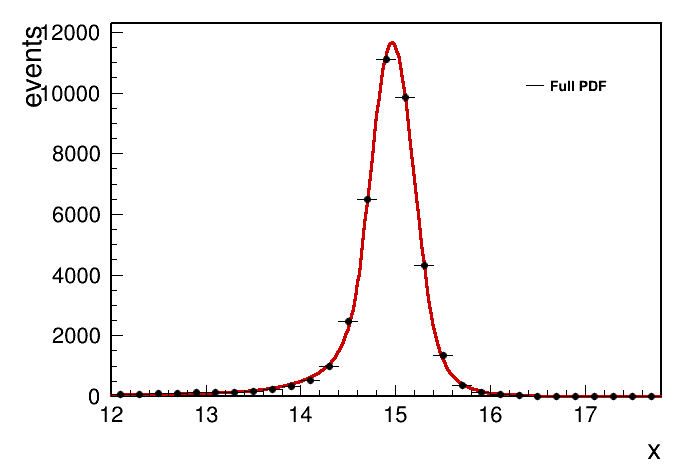
\includegraphics[width=0.5\linewidth]{Figures/8Systematics_figures/Fitting/M15_signal_fit.png}
    \caption{An example fit to the signal shape of a 15\GeV signal with a double crystal ball function. We can see that the signal shape is well described by the functional form fit.}
    \label{fig:sig_fit_15}
\end{figure}

As we only generated signals at a discrete set of mass points at 5\GeV intervals, an interpolation scheme is used to determine the signal shape at intermediate mass points.
This interpolation scheme interpolates the parameters of the double crystal ball fits to estimate their values at each desired mass point.

The interpolation is performed separately for each parameter of Eq.~\ref{eq:dcb} as a function of the
generated resonance mass, and is shown in Fig.~\ref{fig:interp_params}.
The core parameters $\mu$ and $\sigma$, which set the position and width of the resonance and therefore
drive the sensitivity of the search, vary smoothly and monotonically with mass and are interpolated with a
spline through the fitted points.
The tail parameters $\alpha_i$ and $n_i$ are only weakly constrained by the fits at each individual mass
and show no strong mass dependence; they are described by a linear trend, about which the individual fitted
points scatter by an amount comparable to their uncertainties.
Templates are produced on a 0.1\GeV grid, which is finer than the mass resolution everywhere in the search
range, so that every mass hypothesis in the scan is served by a template within a small fraction of
$\sigma$ of its nominal mass.
The signal templates are built over $10 < m_{\mu\mu} < 75$\GeV.
\begin{figure}[h!]
    \centering
    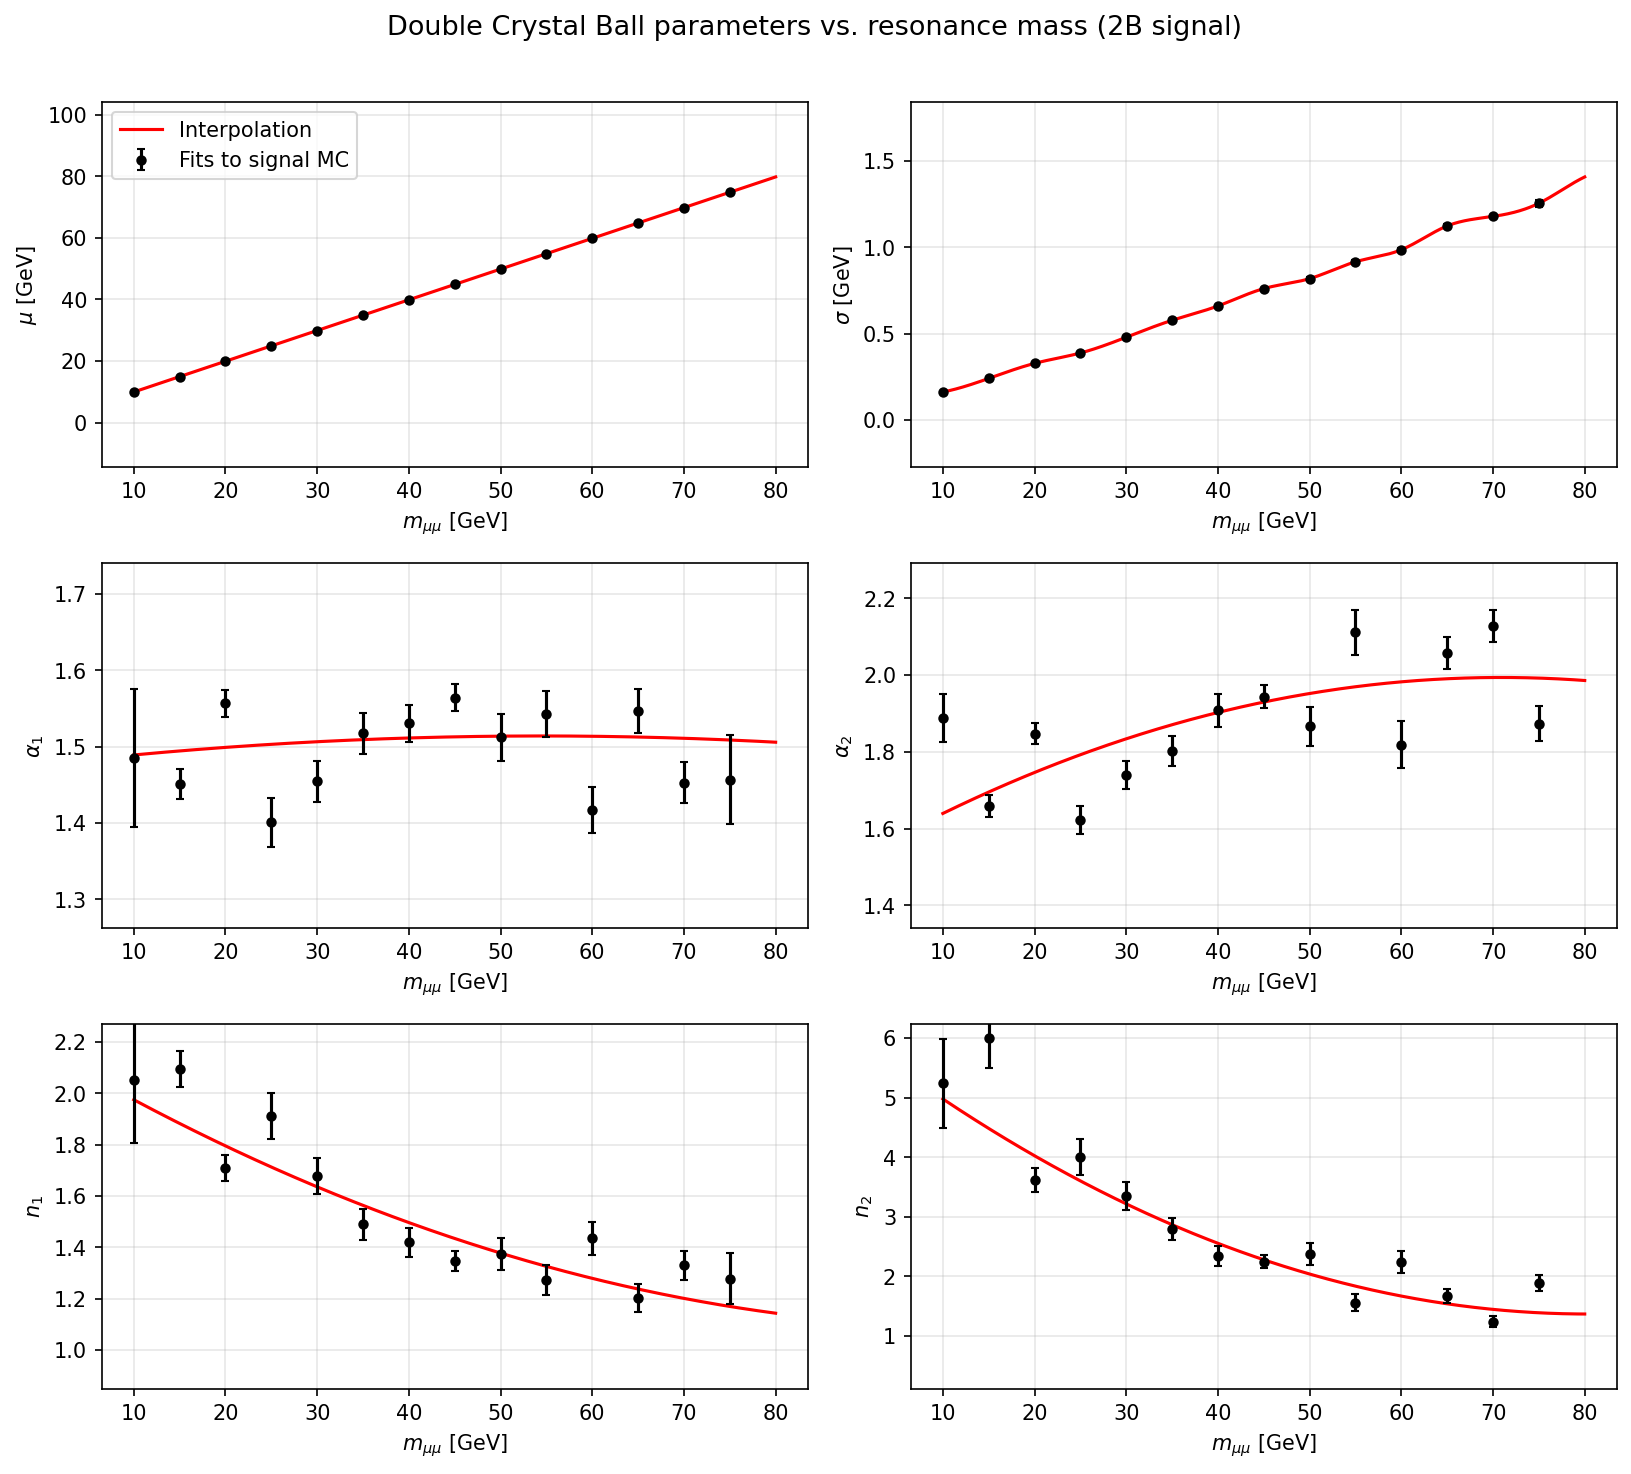
\includegraphics[width=0.95\linewidth]{Figures/8Systematics_figures/Fitting/interp_params_vs_mass.png}
    \caption{Parameters of the double Crystal Ball fits to the simulated signal samples (black points)
    as a function of the generated resonance mass, with the interpolation used to produce templates at
    intermediate masses overlaid (red). The core parameters $\mu$ and $\sigma$ vary smoothly with mass and
    are interpolated with a spline. The tail parameters $\alpha_i$, $n_i$ are weakly constrained at each
    individual mass point and are described by a linear trend. The tail parameters of the lowest mass point
    are essentially unconstrained and their uncertainties extend beyond the plotted range.}
    \label{fig:interp_params}
\end{figure}

The accuracy of the interpolation is assessed with a closure test, shown in
Fig.~\ref{fig:interp_closure}.
One generated mass point (20\GeV) is removed from the set used to build the interpolation, the shape at
that mass is then predicted from the remaining points alone, and the prediction is compared to the true
fit to the withheld sample.
The interpolated core parameters reproduce the true ones to $-0.1\%$ in $\mu$ and $+2.2\%$ in $\sigma$,
while the more weakly constrained tail parameters agree at the level of a few percent to $14\%$.
The resulting shape agrees with the true well across the peak.
Performing the same holdout test on other mass points yielded similar results. 
This test is conservative: withholding a point forces the interpolation across a 10\GeV gap, twice the
5\GeV spacing available in the production configuration.

\begin{figure}[h!]
    \centering
    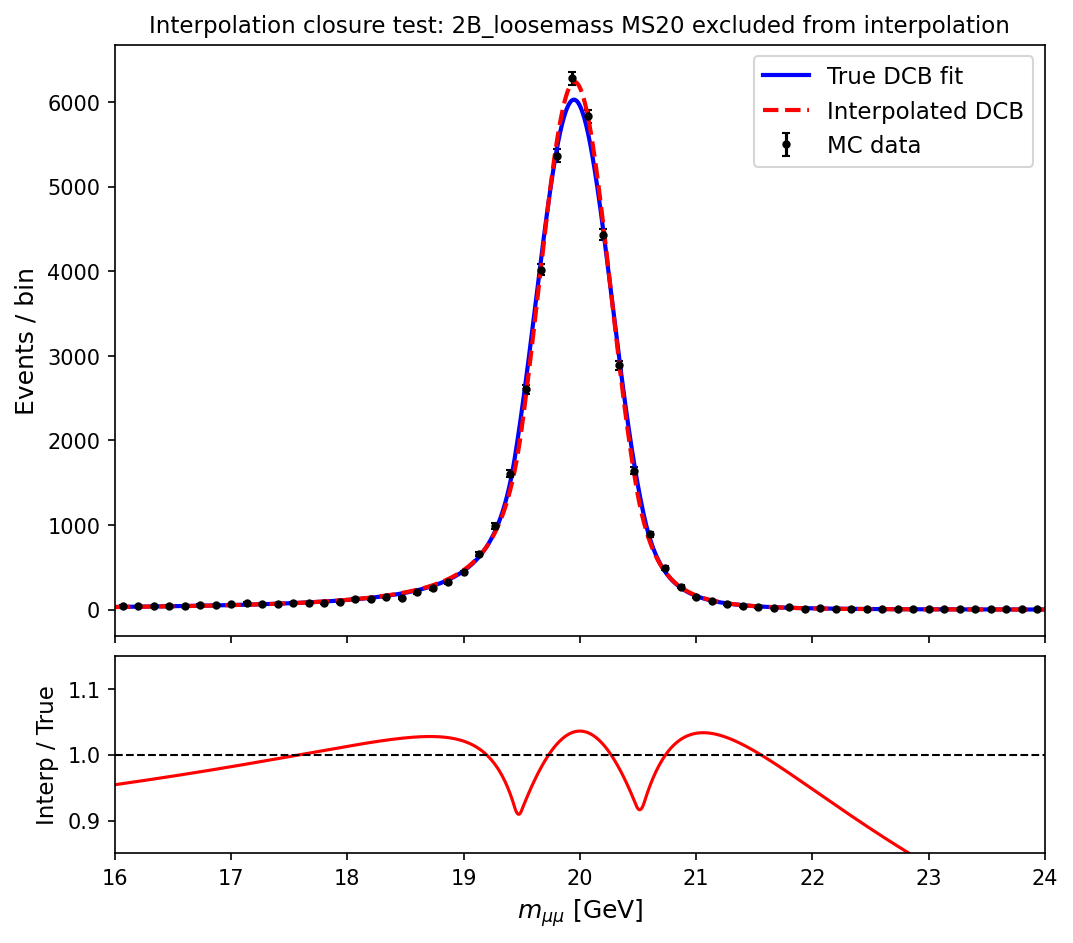
\includegraphics[width=0.6\linewidth]{Figures/8Systematics_figures/Fitting/closure_test_M20.png}
    \caption{Closure test of the signal shape interpolation. The 20\GeV sample is excluded from the set of
    fits used to build the interpolation, and the shape predicted at 20\GeV from the remaining mass points
    (red, dashed) is compared to the direct fit to the 20\GeV simulation (blue, solid) and to the simulated
    events themselves (black points). The lower panel shows the ratio of the interpolated to the true shape.}
    \label{fig:interp_closure}
\end{figure}

\thesis{\subsection{Background Modeling}}
\note{\subsubsection{Background Modeling}}

The background $m_{\mu\mu}$ distribution after the anomaly score selection is expected to be
smoothly varying and approximately monotonically falling across the search range.
However, the exact shape of the background distribution cannot be fully known a priori, as it will depend on the selection made by the anomaly detection algorithm.
Furthermore, because the anomaly detection algorithm learns from the data, and is run separately for each mass window, the selection applied when targeting each mass window will be different.
The background modeling strategy thus needs to be flexible enough to account for these possible variations.
We therefore employ multiple different candidate background shape pdf's, determine the optimal number of parameters for each with an F-test, and then employ discrete profiling \cite{Dauncey:2014xga} to include all of them in the fit.

Discrete profiling, originally developed for the $H \to \gamma \gamma$ analysis, is a method to encode the uncertainty on the signal strength due to the choice of background functional form.
Whenever a background is being fit with an empirical function, there are many choices for functional form choice, all of which may fit the data to a reasonable degree.
Rather than picking a single functional form, discrete profiling fits the data with all functional forms.
Then this family of fits are combined using a new discrete nuisance parameter which encodes which functional form is being used.
The final likelihood scan of the parameter of interest is the minimum negative log likelihood value across different function forms.
Thus at each value of the parameter of interest, the functional form which contributes to the final likelihood is profiled over via the discrete nuisance to determine its optimal value.
This method allows the automated inclusion of these multiple different functional forms and quantifies the uncertainty on the functional form choice.

For each family of functional form, the number of parameters to include still needs to be determined.
For this an F-test is used.
The data is fit multiple times using the functional form with different number of parameters included.
The saturated goodness-of-fit test statistic is assessed for each form.
The starting from the minimal number of parameters, the F-test statistic, based on the difference in the goodness of fit metric between the two fits, is computed to compare against the functional form of one order higher.
The higher order fit is then accepted if it has a p-value less than 0.05.
If the higher order is selected, the procedure is repeated to see if additional orders are warranted.
If the lower order is selected, the procedure terminates.

All functional forms fit a transformed version of the mass variable, rescaled to lie in the range 0 to 1.

\begin{equation}
    x = \frac{m - m_{min}}{m_{max} - m_{min}}
\end{equation}

Where $m_{max}$ and $m_{min}$ are the beginning and end of the sliding window of the mass fit.
For plotting purposes we transform back into the original physical mass scale.

We consider multiple families of functional forms for inclusion in the discrete profiling, following the families included in previous low-mass di-muon analyses (eg EXO-25-019).
\begin{itemize}
    \item Bernstein polynomial: $B_n(x) = \sum_{\nu=0}^{n} \beta_\nu b_{\nu,n}(x)$, where $b_{\nu,n} = \binom{n}{\nu} x^\nu (1-x)^{n-\nu}$
    \item Sum of exponentials: $E_n(x) = \sum_{\nu=1}^{n} a_\nu e^{c_\nu \cdot x}$
    \item Polynomial times exponential: $P_n(x) = e^{c \cdot x} \sum_{\nu=1}^{n} \beta_\nu x^\nu$
    \item Exponential of a polynomial: $Q_n(x) = \exp\!\left( \sum_{\nu=1}^{n} p_\nu x^\nu \right)$
\end{itemize}

The set of orders considered for each family is chosen so that they can describe the background shapes well but do not contain too many additional free parameters which lead to overfitting.

\begin{itemize}
    \item Bernstein polynomial: orders 2--4 (2--4 free parameters)
    \item Polynomial times exponential: orders 1--3 (2--4 free parameters)
    \item Exponential of a polynomial: orders 1--4 (1--4 free parameters)
    \item Sum of exponentials: orders 1--3 (1, 3 and 5 free parameters)
\end{itemize}

Higher order functional forms, which have been used in previous low mass dimuon analyses, were found to be overly flexible and lead to bias for this analysis and are therefore not included.
Studies in MC and our control region confirmed that the functional forms and order choices are sufficient to describe our background. 

\thesis{\subsection*{Signal Extraction}}
\note{\subsection*{Signal Extraction}}

\textbf{Mass scan grid.}
The search is carried out as a scan over discrete resonance mass hypotheses.
The spacing of the scan must be fine enough that a resonance at an arbitrary mass is
close to some hypothesis, since a signal displaced from the hypothesis by much more than the resolution is
poorly described by the corresponding template and the sensitivity is lost.
Because the resolution varies significantly over the search range, the grid is instead spaced by the local
resolution.
Starting from the low edge of the range, each successive tested mass point is added at value of $\sigma(m)$ away from 
the previous mass point. This candidate mass value is then rounded down to match the 0.1 \GeV signal template spacing.
Rounding down rather than to the nearest template.

The resulting grid contains 119 mass hypotheses between 13.8 and 75.0\GeV, and is shown in
Fig.~\ref{fig:scan_grid}.
The step grows from 0.2\GeV at the bottom of the range, where $\sigma = 0.21$\GeV, to 1.1\GeV at the top,
where $\sigma = 1.22$\GeV.

Because the anomaly detection is trained separately in each of the 26 overlapping 5\GeV wide windows, whose
centres run from 15 to 77.5\GeV in steps of 2.5\GeV, a given mass hypothesis could in principle be fit in
more than one window, using a different selection each time.
To avoid fitting the same hypothesis more than once, each hypothesis is assigned to the single window whose
centre is closest to it.
Each window therefore owns a contiguous band of $\pm 1.25$\GeV about its centre, and these bands tile the
search range without overlap or gaps.


\textbf{Fit window and binning}
A window around the searched for resonance mass is constructed for inclusion in the fit.
The window should be wide enough such that the background can be adequately constrained by the sideband regions.
But not so large that the distribution becomes difficult to model.
Because the mass resolution varies significantly across the search range, the window and the
binning are defined in units of the local signal width $\sigma$, taken from the interpolated signal
template, rather than as fixed intervals in \GeVns.

The nominal configuration uses a window of $\pm 7\sigma$ around the mass hypothesis, with bins of size 
$0.5\sigma$.
This configuration was found to lead to stable and unbiased fits. 
It was tested that making smaller bins did not improve the constraint on the signal strength.
For each fit the goodness of fit is evaluated from the $\chi^2$/ndof of the signal plus background fit,
where the number of degrees of freedom accounts for the parameters actually floating in the fit, the
background normalization, and the signal strength.

In some cases the goodness of fit of the fit is poor, $p < 0.05$. 
Since the exact shape of the distributions we will be fitting is unknown a priori, we developed an automated re-fitting procedure to handle this. 
If the goodness of fit is poor, the $\pm 7 \sigma$ window is shrunk in steps of $0.5\sigma$ and the fit repeated. 
This continues until an acceptable goodness of fit $p > 0.05$ is achieved. 
The minimum allowed window is $\pm 4\sigma$. 
If the $\pm 4\sigma$ window is reached and the goodness of fit is still poor, the bin size is increased in steps of $0.1\sigma$ up to a maximum of
$1.0\sigma$ and the window scan is repeated.
A poor goodness of fit at fine binning can be caused by a narrow statistical fluctuation landing in a
single bin rather than by a genuine failure of the background model, but coarser bins cost signal
resolution, so they are only used when the entire window scan fails.
In the rare case that no combination gives an acceptable goodness of fit, the attempt with the highest
goodness of fit p-value is retained and reported and flagged for inspection. 
Windows are additionally truncated at the boundaries of the available mass range.

An example fit is shown in Fig.~\ref{fig:example_dimuon_fit}.

\begin{figure}
    \centering
    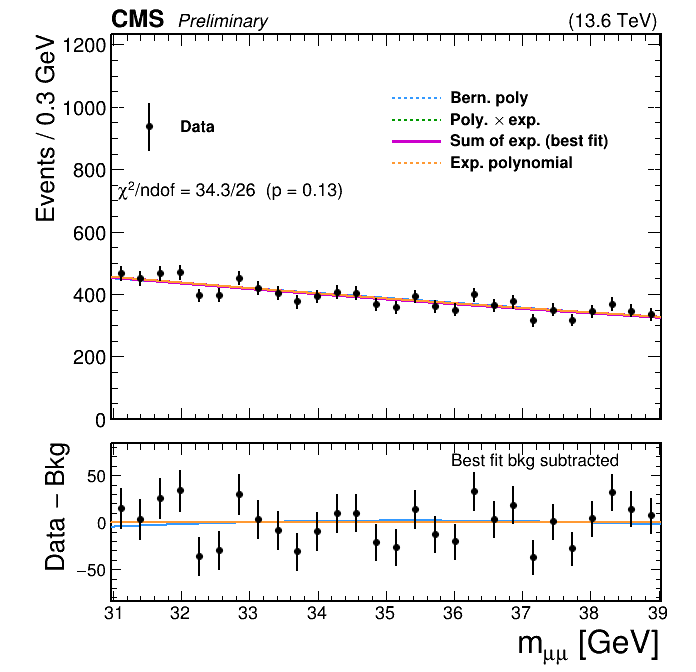
\includegraphics[width=0.6\linewidth]{Figures/8Systematics_figures/Fitting/fit_example.png}
    \caption{An example background-only fit to the di-muon mass spectrum in simulation, at a mass
    hypothesis of 35\GeV. All four families of functional forms entering the discrete profiling are shown,
    with the form selected by the fit drawn as a solid line. The lower panel shows the data minus the best
    fit background. The goodness of fit based on the $\chi^2$/ndof is good and no excess is present, as
    expected.}
    \label{fig:example_dimuon_fit}
\end{figure}

\thesis{\subsection{Validation of the Fit Procedure}}
\note{\subsubsection{Validation of the Fit Procedure}}
\label{sec:fit_validation}

The fit procedure is validated on simulated background.
Since we do not know the exact mass shapes after the application of the anomaly score on data, we first do tests on the background 
distribution prior to the anomaly score cut, ie assuming the mass shape is unchanged by the anomaly score cut. 
Because the search applies an anomaly score selection with an efficiency of approximately 1\% before the
mass fit, and we have approximately 3 times more data than MC events, the validation is performed on random 3\% subsamples of the MC.
This tests the fit on the same statistics it will encounter in the real application to data. 
Twenty statistically independent subsamples are drawn, and each is fit at mass hypotheses of 15, 35, 55 and
75\GeV using the full procedure described above, including the adaptive window and binning.

The background-only goodness of fit is shown in Fig.~\ref{fig:gof_ensemble}.
The mean $\chi^2$/ndof is 0.92, 0.86, 1.08 and 0.94 at 15, 35, 55 and 75\GeV respectively, with no
pathological outliers, indicating that the set of functional forms is able to
describe the background shape.

\begin{figure}[h!]
    \centering
    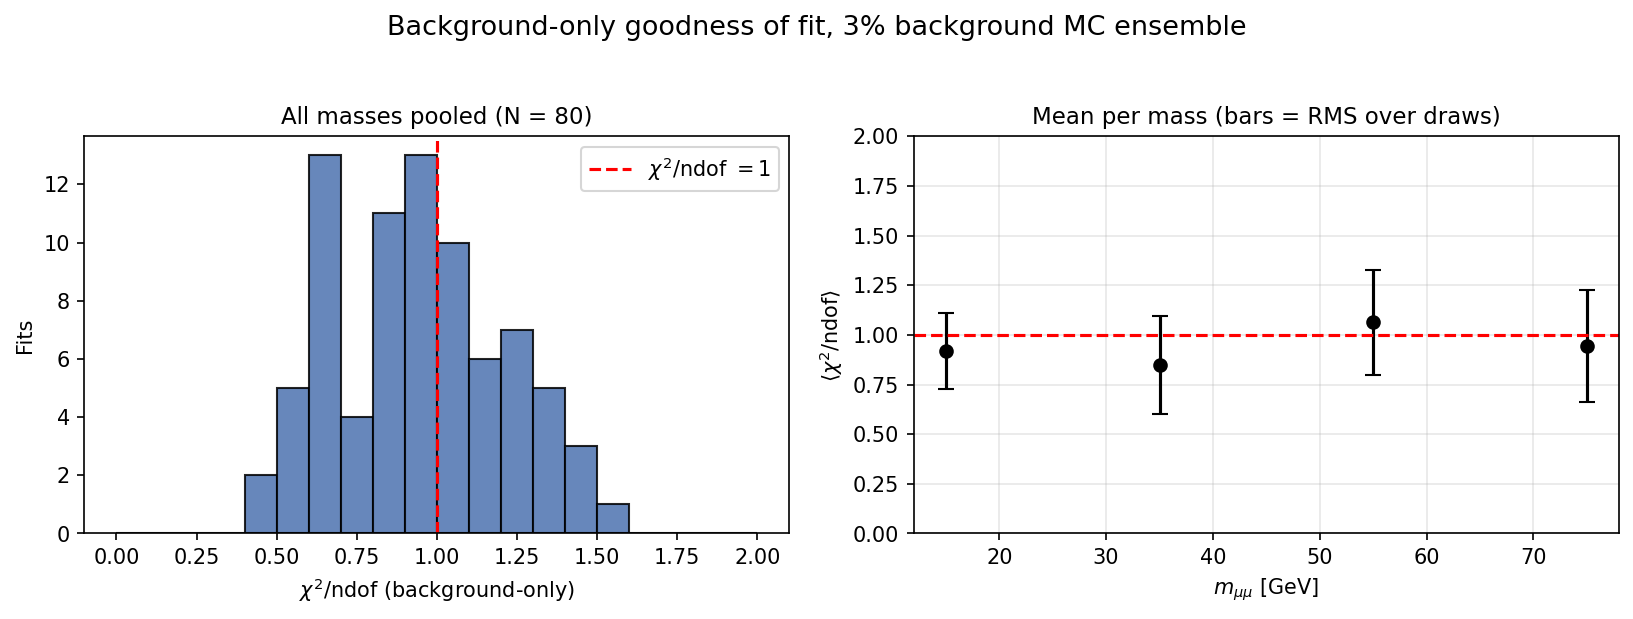
\includegraphics[width=0.95\linewidth]{Figures/8Systematics_figures/Fitting/gof_ensemble.png}
    \caption{Background-only goodness of fit over an ensemble of twenty independent subsamples containing
    3\% of the background simulation. Left: the $\chi^2$/ndof of all fits, pooled over the four mass
    hypotheses. Right: the mean $\chi^2$/ndof at each mass hypothesis, with bars indicating the spread over
    the twenty draws.}
    \label{fig:gof_ensemble}
\end{figure}

A further test using pseudo experiments is performed to properly test the bias of the fit.
Sampling subsets of the simulation directly is not adequate for this purpose, because every subsample
inherits the statistical fluctuations of the finite parent sample, which are then indistinguishable from a
bias of the method.
Toys generated from fits to the background shape are therefore used instead.

At each mass hypothesis the full background simulation is fit with the procedure described above, which
yields a workspace containing all four families of functional forms, each at its F-test selected order with
its parameters at the full-simulation best fit.
Pseudo-data are then generated from each of these four functional forms in turn, with the background
normalization set to the 3\% of the full simulation statistics, so that the toys carry
the statistical precision of the search.
Each toy is fit with the complete discrete profiling envelope, exactly as the search fits the data, so that
the functional form used to fit a toy is chosen by the fit itself and is not restricted to the one that
generated it.
This measures the bias induced by the choice of background functional form, which is the quantity discrete
profiling is designed to control, and by construction it is insensitive to fluctuations of the simulation.
A signal is injected at a strength corresponding to zero, approximately two, and approximately five
standard deviations, to test both whether the fit manufactures a signal where none exists and whether it
recovers a genuine one without bias.
One hundred toys are generated for each combination of mass (15, 35, 55, 75 \GeV), generating function (4 families) and injected signal
strength (0, 2 and 5 $\sigma$). 

The resulting median pulls, $(r_{\mathrm{fit}} - r_{\mathrm{gen}})/\sigma_r$, are shown in
Fig.~\ref{fig:bias_toys}.
The widths of the pull distributions lie between 0.86 and 1.15, close to unity, confirming that the
uncertainty on the extracted signal strength is reasonably estimated.
At 15, 35 and 55\GeV the median pull lies between $-0.38$ and $+0.02$ for every generating function and
every injected signal strength, comfortably within the conventional acceptance criterion of
$|\mathrm{median\ pull}| < 0.5$, and no additional systematic uncertainty for the choice of background
functional form is required in this range.

At 75\GeV a small coherent negative offset is observed, with a median pull between $-0.63$ and $-0.27$.
We are investigating if this related to edge effects of our fitting range (80 \GeV).

\begin{figure}[h!]
    \centering
    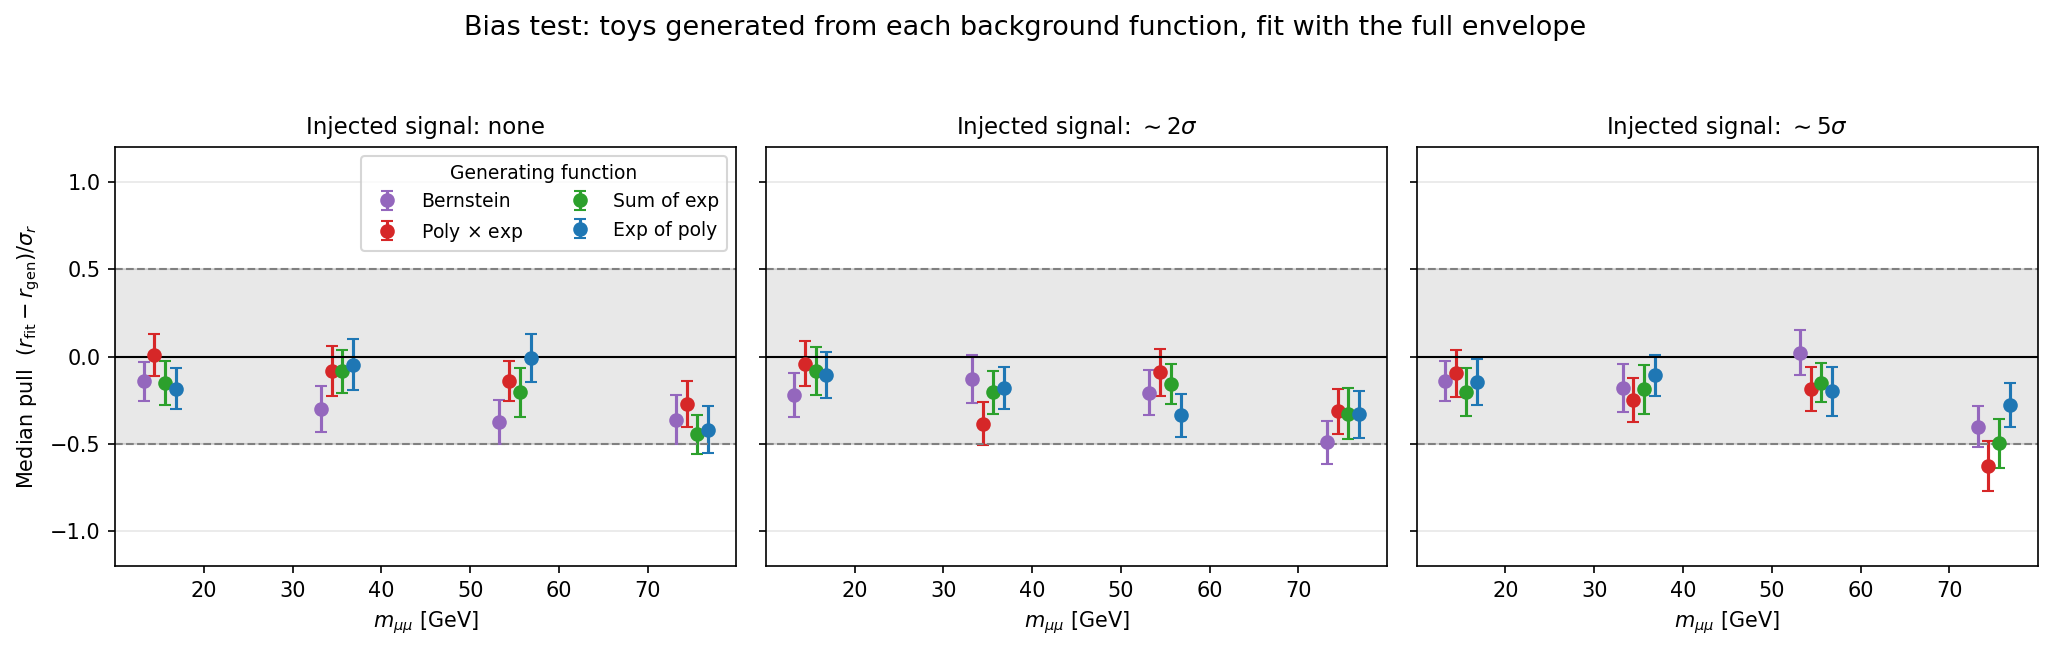
\includegraphics[width=0.98\linewidth]{Figures/8Systematics_figures/Fitting/bias_toys.png}
    \caption{Median pull of the extracted signal strength, $(r_{\mathrm{fit}} -
    r_{\mathrm{gen}})/\sigma_r$, for toys generated from each of the four background functional forms
    (colours) and fit with the complete discrete profiling envelope. The three panels correspond to no
    injected signal and to injected signals of approximately two and five standard deviations. One hundred
    toys are used per point, and the error bars show the uncertainty on the median. The shaded band
    indicates the conventional acceptance criterion $|\mathrm{median\ pull}| < 0.5$. Points are offset
    horizontally by generating function for legibility.}
    \label{fig:bias_toys}
\end{figure}

\subsubsection{Full-Range Scan on the Post-Selection Signal-Region Simulation}
\label{sec:srmc_scan}

The tests above use background simulation prior to the anomaly score selection, since the exact mass shape on data after the anomaly score cut is unknown a priori.
This demonstrates the fitting framework can handle the background shape if there is no sculpting.
However it is important to verify that the anomaly score cut indeed does not cause any sculpting. 
This is checked by running the full procedure on simulated signal-region background processed through the actual CATHODE pipeline -- the same generative model, classifier, and anomaly selection used on data -- providing the closest available proxy of the real analysis chain.
The bump-hunt fit is performed at 97 mass hypotheses between 13.8 and 75.0\GeV, distributed over 19 mass windows.
A narrow band, 47.5--52.5\GeV, is excluded from the scan: this is the region in which the mass-binned Drell-Yan samples change boundary, and we found that our procedure was sensitive to artifacts related to the difference between these two different Drell-Yan samples, leading to strange effects right at this 50 \GeV boundary. 
We therefore exlcude this region, every mass hypothesis whose nominal $\pm7\sigma$ fit window would overlap it is dropped.

The background-only goodness of fit is summarized in Fig.~\ref{fig:srmc_bkg_gof}, alongside the goodness of fit of the signal-plus-background fit actually used to extract the result.
Across the 97 fits the mean background-only $p$-value is 0.48 and the median $\chi^2/\mathrm{ndof}$ is 1.01, consistent with an adequate background description.
Three fits fall below $p = 0.05$ for the background-only model; in every one of these the signal-plus-background fit recovers a good description ($p \geq 0.05$), and inspection of the residuals shows diffuse bin-to-bin fluctuations rather than a coherent peaking structure, so none indicate a real feature.

\begin{figure}[h!]
    \centering
    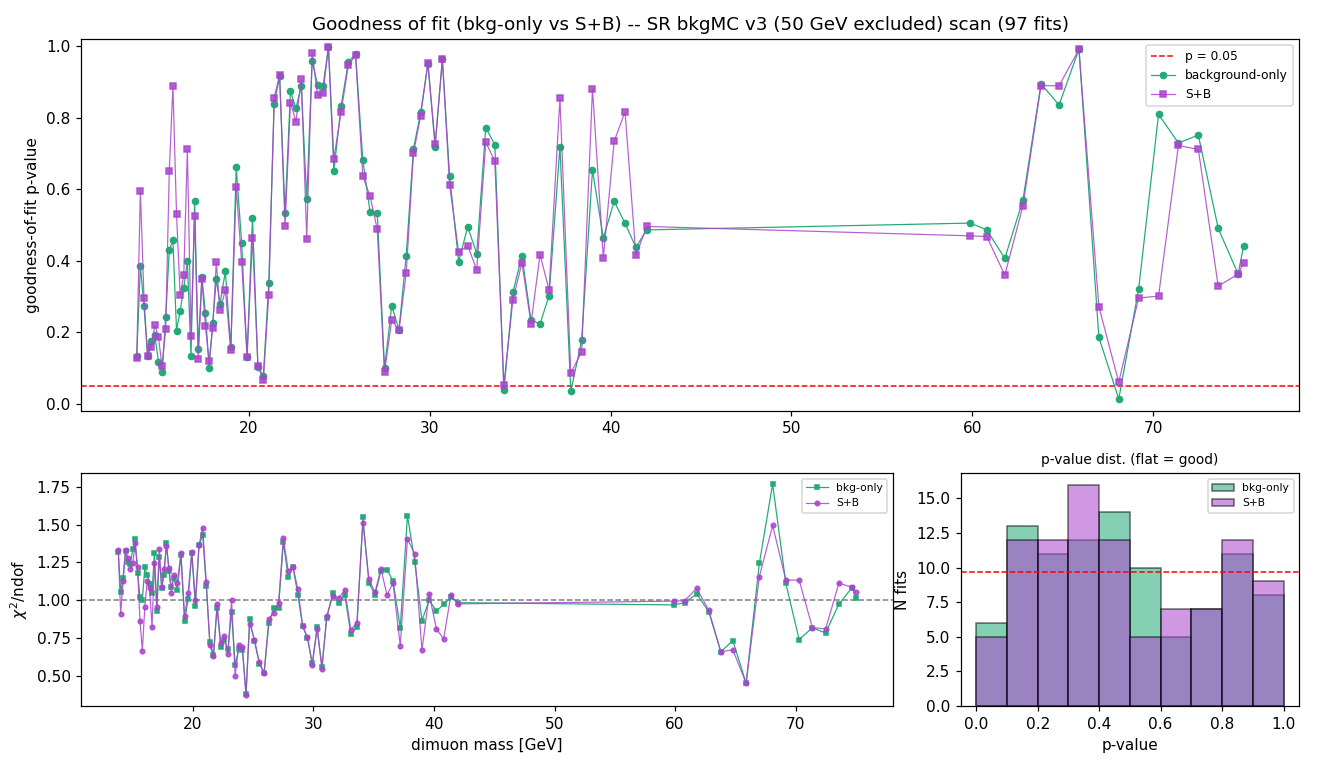
\includegraphics[width=0.95\linewidth]{Figures/8Systematics_figures/Fitting/srmc_scan_bkg_gof.png}
    \caption{Goodness of fit over the 97 mass hypotheses of the signal-region background simulation scan, comparing the background-only fit (green) to the signal-plus-background fit (magenta) used to extract the result.
    Top: the goodness-of-fit $p$-value as a function of the di-muon mass hypothesis, with the $p = 0.05$ threshold indicated.
    Bottom left: the corresponding $\chi^2/\mathrm{ndof}$ for both fits.
    Bottom right: the $p$-value distributions for both fits.}
    \label{fig:srmc_bkg_gof}
\end{figure}

The background functional form and fit window chosen by the adaptive procedure are summarized in Fig.~\ref{fig:srmc_fit_config}.
As in the same-sign control region, the number of free background parameters selected by the F-test is low: a single parameter suffices for 56 of the 97 fits, two for 30, three for 9, and four for the remaining 2.
The adaptive window shrinks below its nominal $\pm7\sigma$ at only 2 of the 97 mass hypotheses.

\begin{figure}[h!]
    \centering
    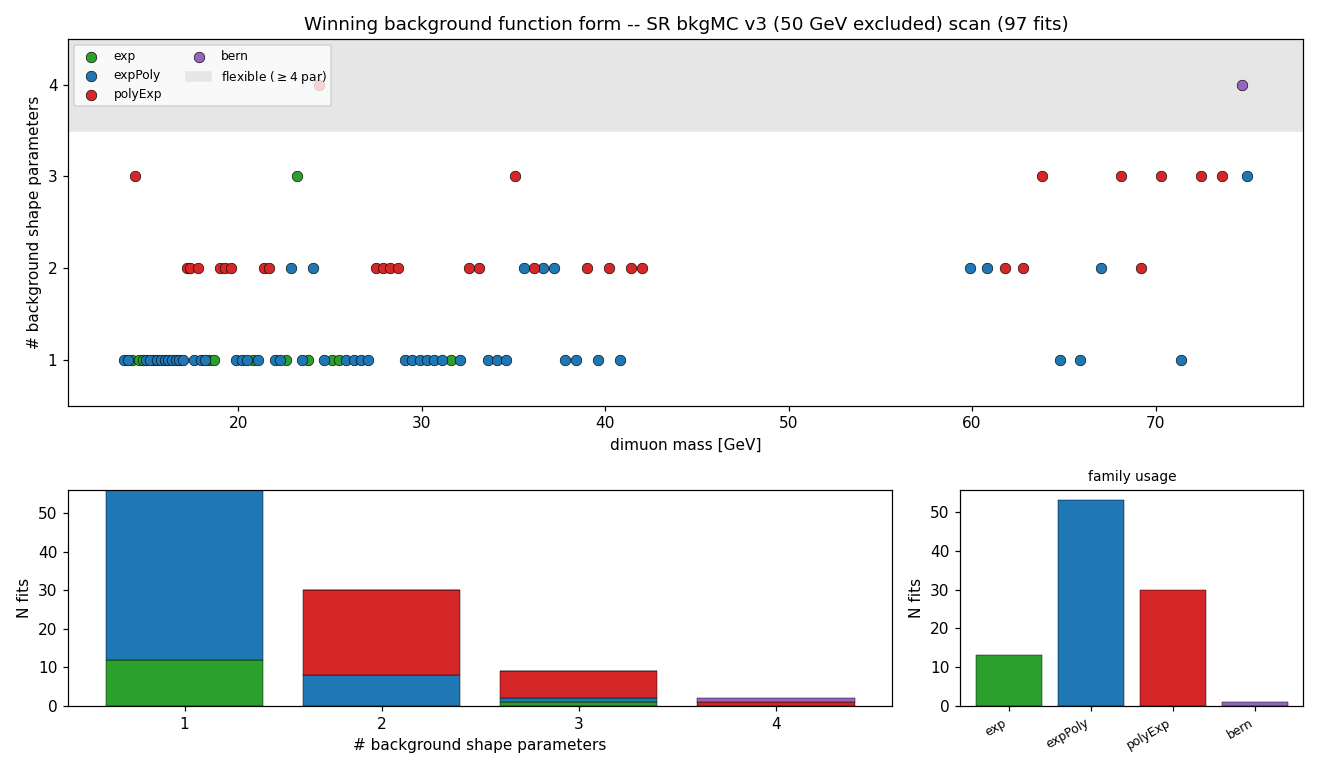
\includegraphics[width=0.49\linewidth]{Figures/8Systematics_figures/Fitting/srmc_scan_func_forms.png}
    \hfill
    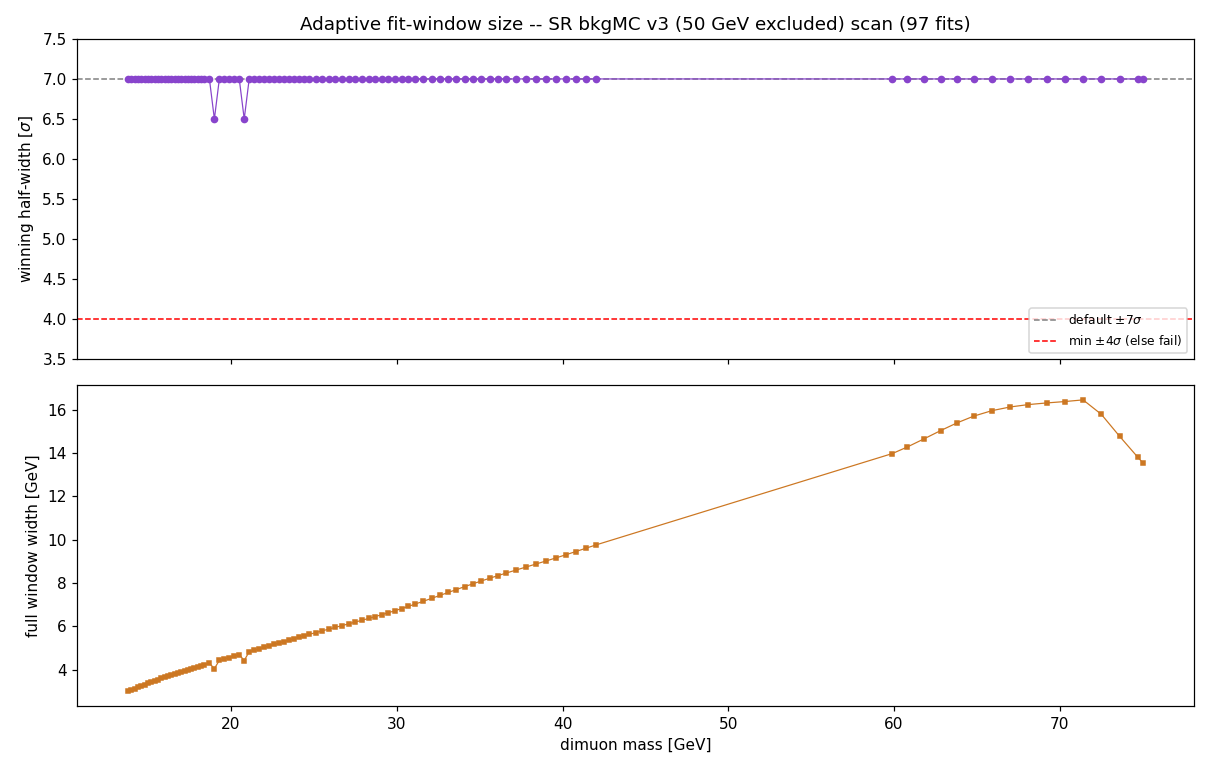
\includegraphics[width=0.49\linewidth]{Figures/8Systematics_figures/Fitting/srmc_scan_window_sizes.png}
    \caption{Fit configuration selected by the adaptive procedure across the 97 mass hypotheses of the signal-region background simulation scan.
    Left: the winning background functional form as a function of the di-muon mass hypothesis, coloured by family, with the number of free background parameters on the vertical axis.
    Right: the winning fit-window half-width in units of the local resolution $\sigma$ (top) and the corresponding full window width in \GeVns\ (bottom).}
    \label{fig:srmc_fit_config}
\end{figure}

The local significance of the fitted signal yield at each mass hypothesis is shown in Fig.~\ref{fig:srmc_significance}.
The significances scatter symmetrically about zero and lie between $-3.1\sigma$ and $+2.7\sigma$ across the search range, with the largest excursion, $-3.1\sigma$, at 15.8\GeV.
Given the 97 correlated hypotheses tested, none of these fluctuations constitute a globally significant excess.

\begin{figure}[h!]
    \centering
    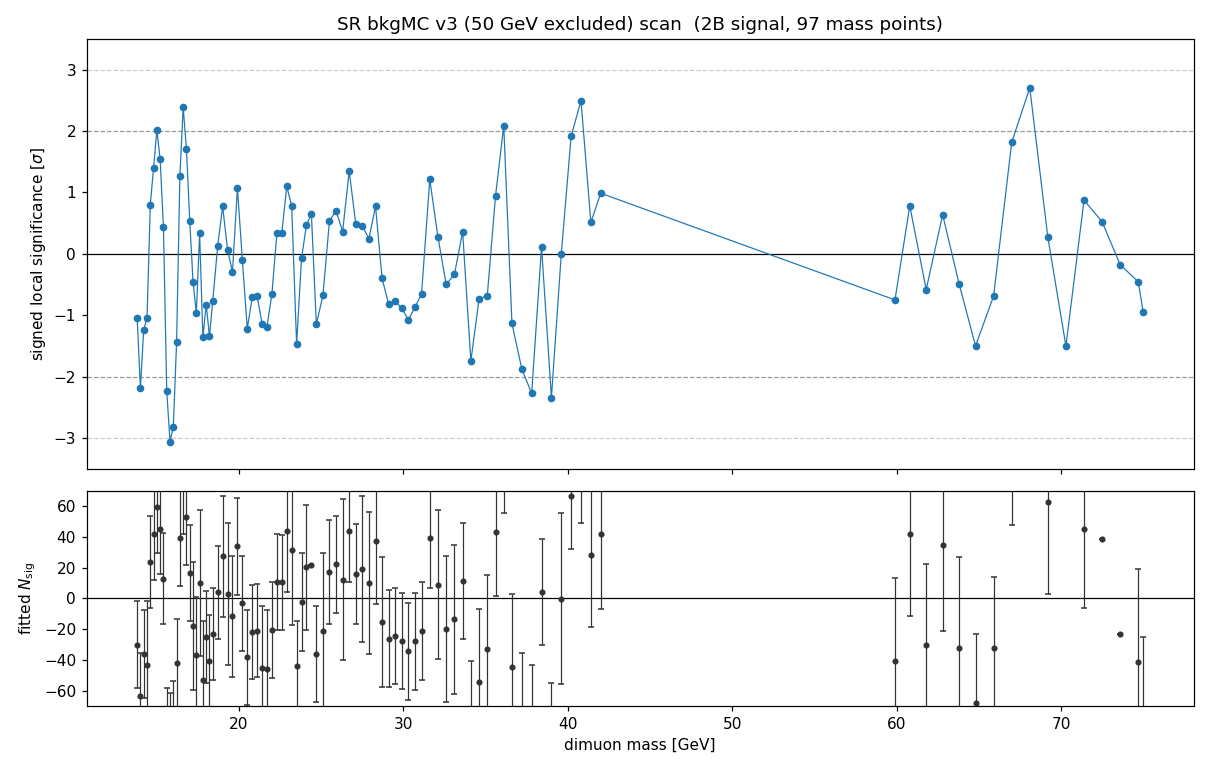
\includegraphics[width=0.95\linewidth]{Figures/8Systematics_figures/Fitting/srmc_scan_significance.png}
    \caption{Signed local significance of the fitted signal yield (top) and the fitted signal yield $N_\mathrm{sig}$ with its uncertainty (bottom) as a function of the di-muon mass hypothesis, for the 97 fits of the signal-region background simulation scan.
    The significances scatter symmetrically about zero and lie between $-3.1\sigma$ and $+2.7\sigma$ over the full range.}
    \label{fig:srmc_significance}
\end{figure}

Together with the same-sign control region scan of Section~\ref{sec:cr_pipeline_validation}, this confirms that the CATHODE pipeline does not sculpt artificial structure in the $m_{\mu\mu}$ spectrum when applied to background alone, in either a data-driven or simulation-based signal-free sample.